\documentclass[a4paper]{article}
\usepackage{hyperref}
\usepackage{graphicx}
\graphicspath{ {./images/} }
  
\begin{document}
  \begin{titlepage}
    \begin{center}
      \vfill
      \textbf{\huge{Skyrmion Trajectory Prediction \\ \vspace{5pt} Progress Update}} \\
      \vfill
      \hrule
      \vspace{5pt}
      \textbf{\large{University of Manchester}} \\
      \large{Chen Bo Calvin Zhang (10403253)} \\
      \large{Computer Science and Mathematics} \\
      \large{July 22nd 2020} \\
      \vspace{5pt}
      \hrule
      \vfill
    \end{center}
  \end{titlepage} 
  
  \tableofcontents
  
  \newpage
  \section{Experiment 1}
  In the first experiment, I am using linear regression to predict the next frame given the previous one. I do not think there are any updates on this experiment since our last meeting.

We can see the results in figure \ref{fig:exp1} (this is just skyrmion 0). It seems to fit the ground truth very well on the training set (on the left of the gree line) and it seems to be giving quite a good fit on the test set (on the right of the green line) as well. As we discussed some time ago, this shows that there is a linear relationship between the positions of skyrmions in one frame and their position in the next frames. Of course, this was just an initial experiment as it is not really practical for our purposes of predicting trajectories given a few initial positions.

\begin{figure}[h]
  \centering
  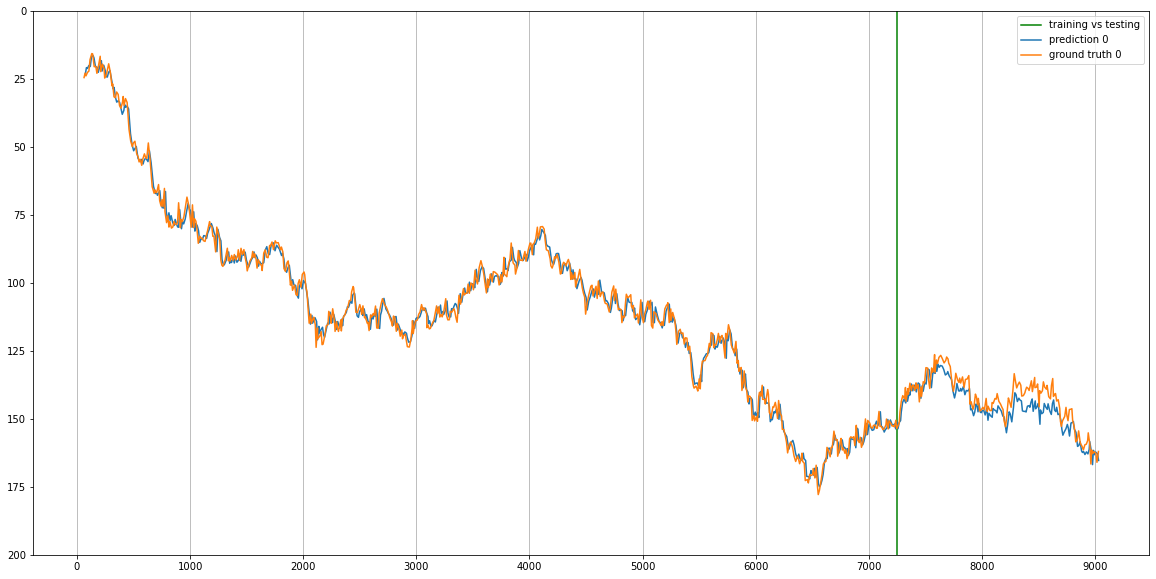
\includegraphics[width=\textwidth]{exp 1}
  \caption{Experiment 1}
  \label{fig:exp1}
\end{figure}

In experiment 1, I also tried using polynomial regression with l2 regularisation, because it was overfitting the training data, but even with regularisation it still overfits and performs very poorly on the test set. The results can be seen in figure \ref{fig:exp1poly} (this is just skyrmion 0).

\begin{figure}[h]
  \centering
  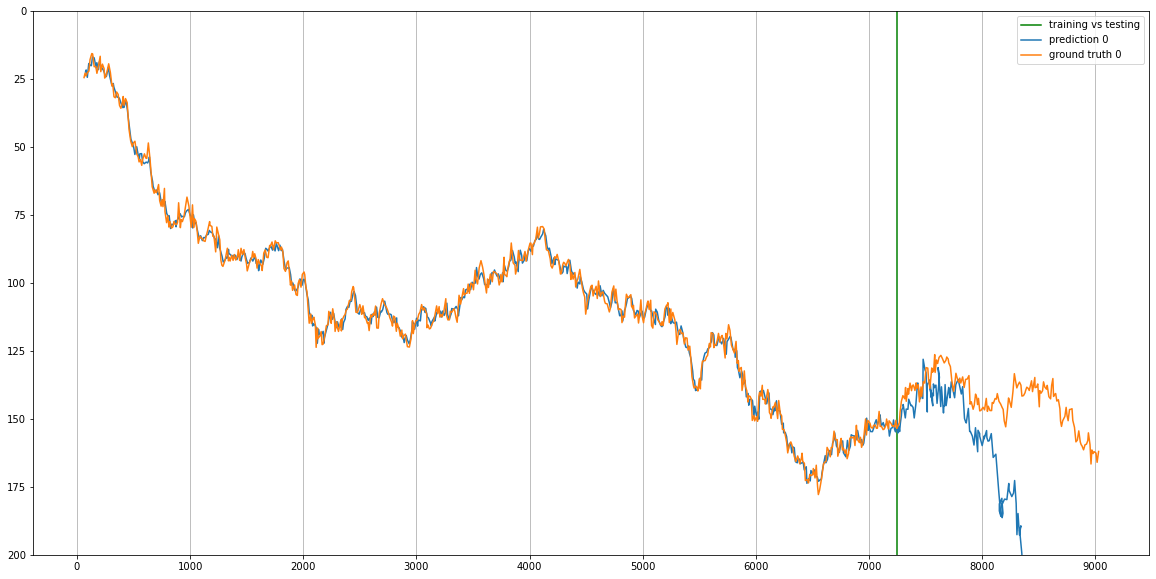
\includegraphics[width=\textwidth]{exp 1 poly}
  \caption{Experiment 1 Poly}
  \label{fig:exp1poly}
\end{figure}

\section{Experiment 3}
This was probably one of the most interesting experiments. The data is organised as in experiment 1 (i.e. given one frame, I want to predict the next one), but in this experiment, I want to try to predict trajectories with fewer data. What I am doing is basically taking the first frames and predicting the second frame. With the prediction of the second frame, I predict the third frame, and so on. Of course, this makes the prediction get further and further from the ground truth at every subsequent prediction. Figure \ref{fig:exp3} shows how it performs on training and test set. The fact that the blue prediction stops much earlier than experiment 1 is due to the fact that I am using much smaller sets for training and testing. As you can see, it still performs okay on both training and testing.

\begin{figure}[h]
  \centering
  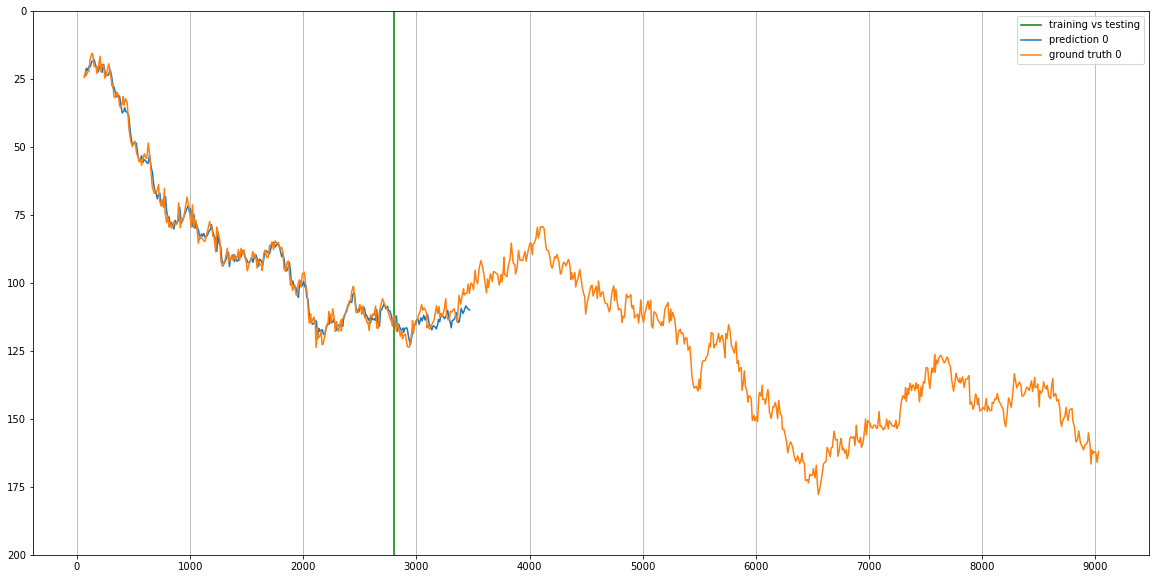
\includegraphics[width=\textwidth]{exp 3}
  \caption{Experiment 3}
  \label{fig:exp3}
\end{figure}

In figure \ref{fig:exp3succ} you can see the results of predicting successively and, as expected, the prediction gets further and further from the truth. We discussed using an observer, but I am really not sure how to implement this. One idea I had, was to measure $RMSE$ and $R^2$ every time I predict and if both are over a certain threshold, instead of using the previous prediction to get the next frames, I can use the ground truth. This would effectively use fewer data, but as you can see from the image, the predictions would not be too precise anyways as after just a few frames, hence making us use quite a bit of data.

\begin{figure}[h]
  \centering
  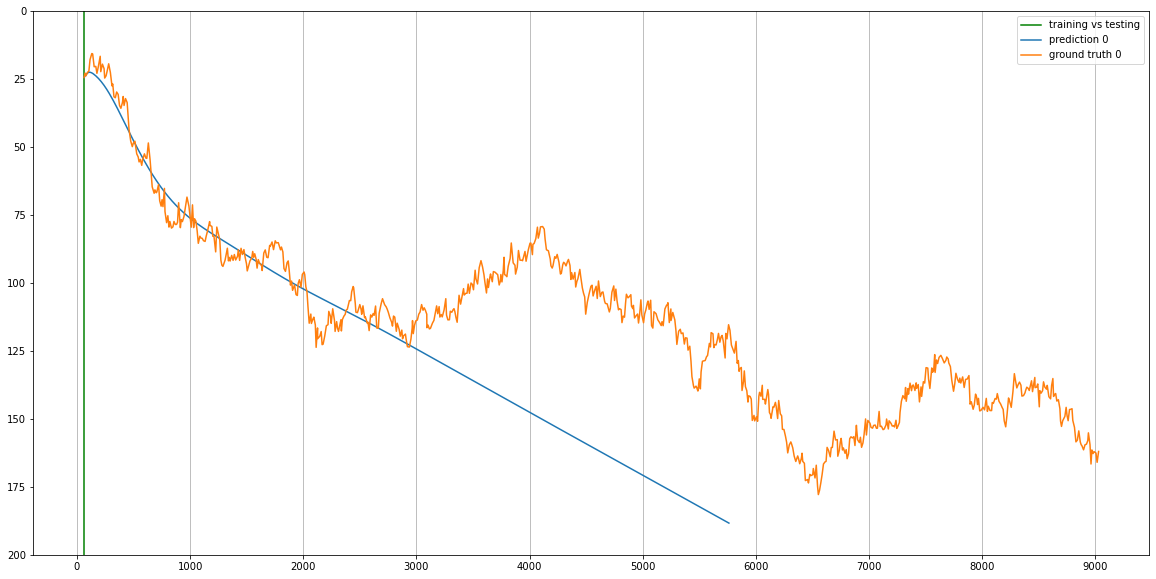
\includegraphics[width=\textwidth]{exp 3 successice}
  \caption{Experiment 3 Successive}
  \label{fig:exp3succ}
\end{figure}

\section{Experiment 4}
In all the following experiments, the plotting problem has been solved.

In this experiment, half of the particles are randomly chosen for training and the other half is used for testing (of course, one particle is left out as the is an odd number of skyrmions). This is again somewhat similar to experiment one as we are predicting the next frame given the previous one (ground truth) and again we can see that there is a linear relationship between one frame and the next. The results of this experiment can be seen in figures \ref{fig:exp4train} and \ref{fig:exp4test}. One thing we can see is that it fits the training set quite well, but it seems to be slightly shifted upwards for the testing set, but it does capture the behaviour from one frame to the next quite well.

\begin{figure}[h]
  \centering
  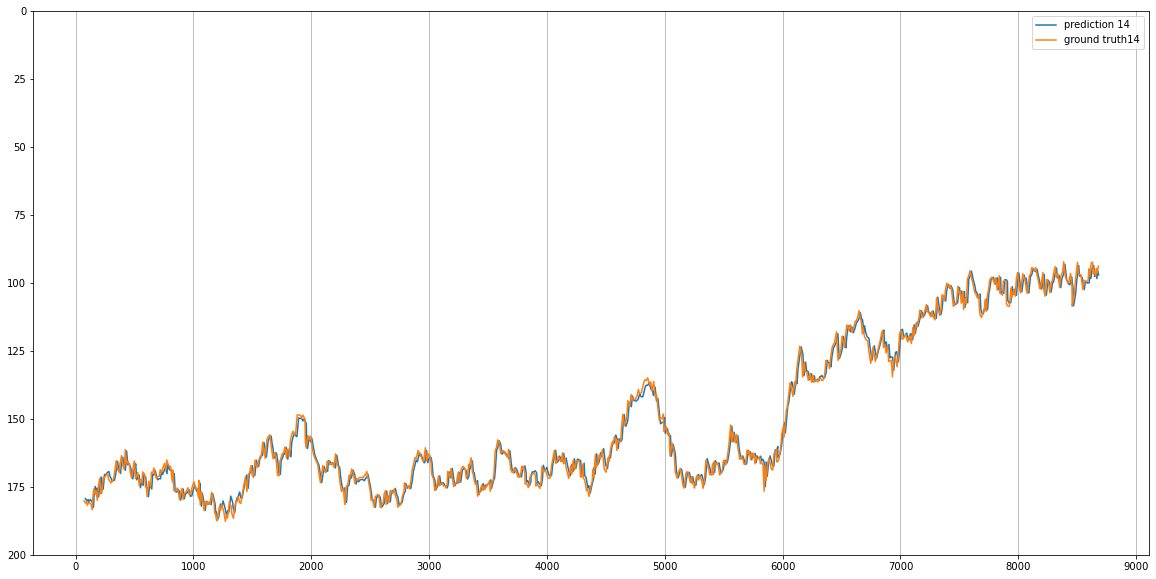
\includegraphics[width=\textwidth]{exp 4 train}
  \caption{Experiment 4 Training}
  \label{fig:exp4train}
\end{figure}

\begin{figure}[h]
  \centering
  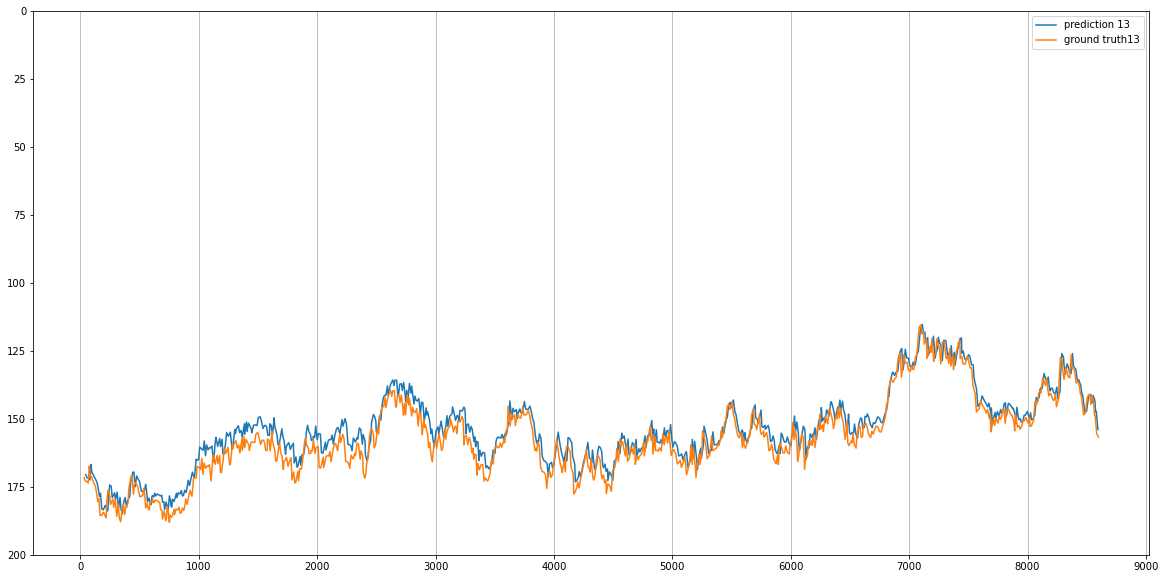
\includegraphics[width=\textwidth]{exp 4 test}
  \caption{Experiment 4 Test}
  \label{fig:exp4test}
\end{figure}

\section{Experiment 5}
This experiment is set in the same way as experiment, but in this case the training and testing sets are not randomly chosen, but in the first part, I use the top half for training and the bottom for testing and vice versa in the second part.

Here again we can see that in both the test sets there is a shifting, but the general behaviour is captured.

\begin{figure}[h]
  \centering
  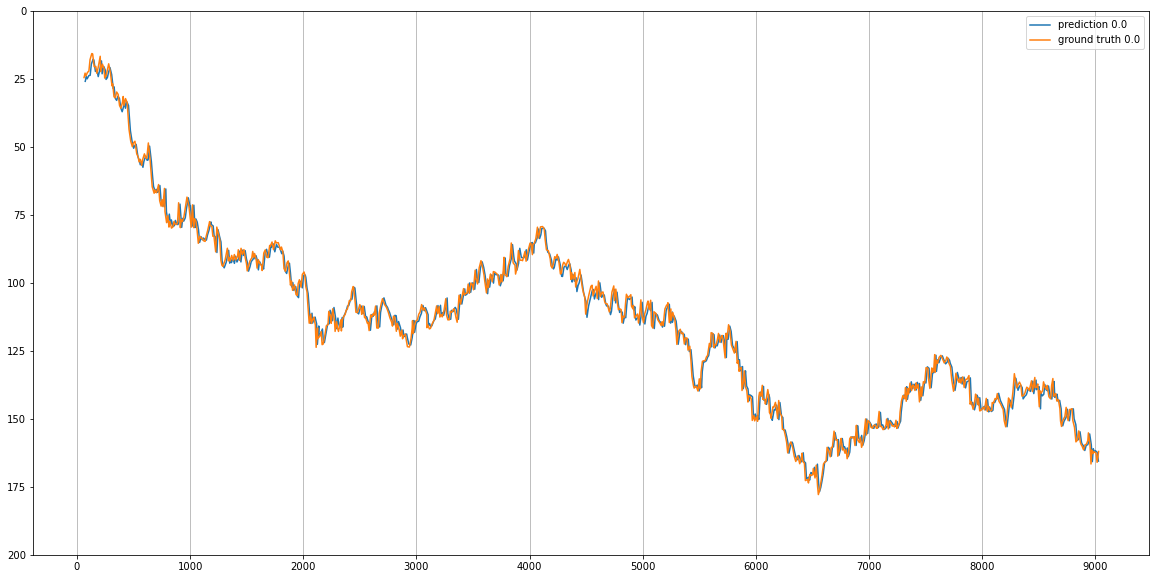
\includegraphics[width=\textwidth]{exp 5 train top}
  \caption{Experiment 5 with top particles as training set (shown) and bottom particles as testing set}
\end{figure}

\begin{figure}[h]
  \centering
  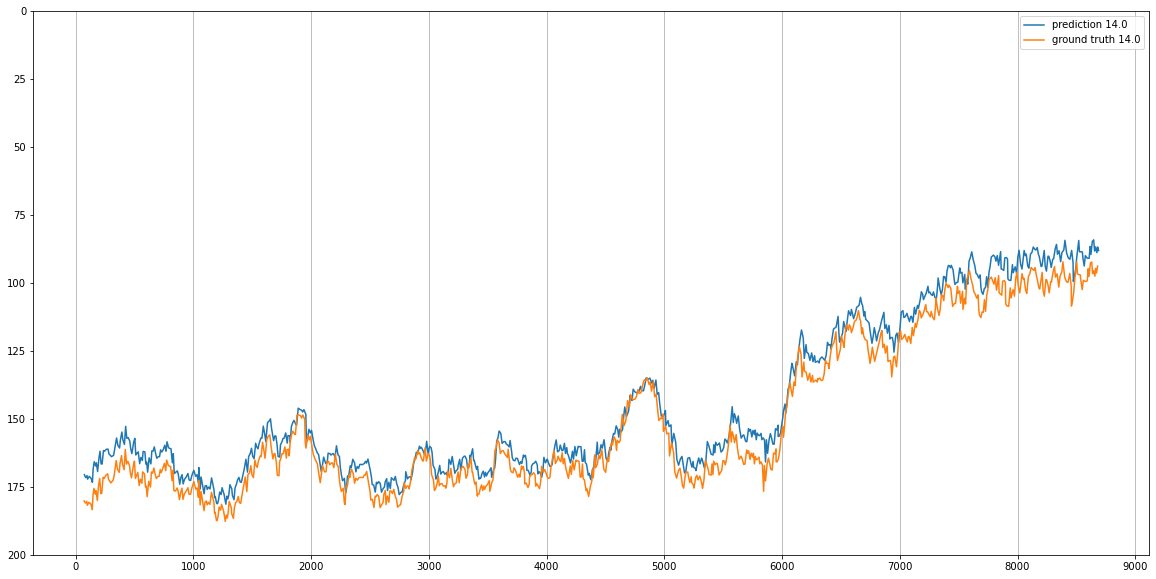
\includegraphics[width=\textwidth]{exp 5 test bot}
  \caption{Experiment 5 with top particles as training set and bottom particles as testing set (shown)}
\end{figure}

\begin{figure}[h]
  \centering
  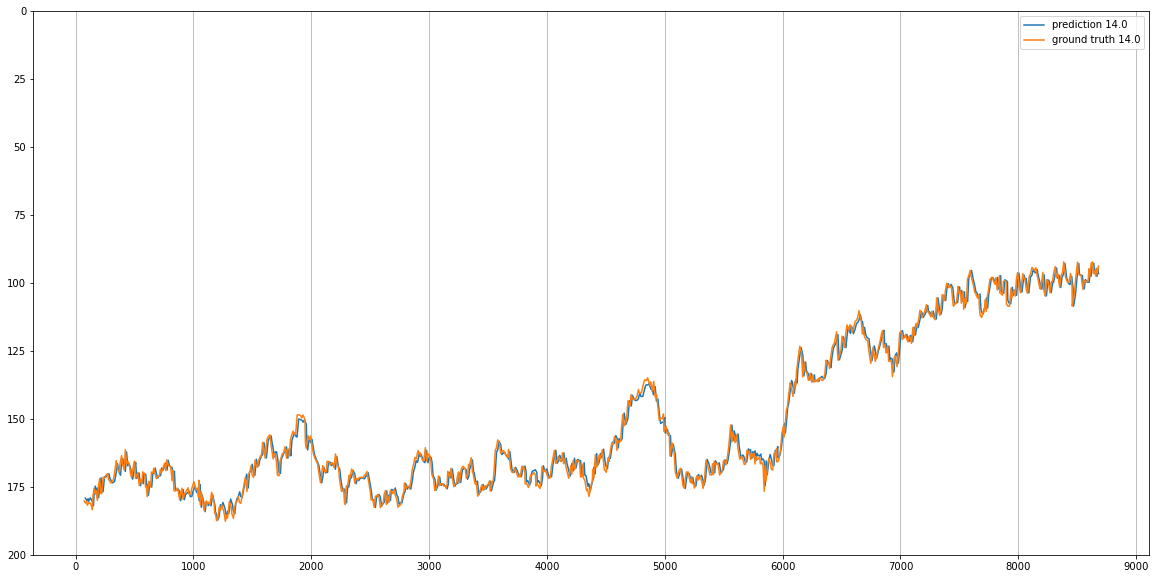
\includegraphics[width=\textwidth]{exp 5 train bot}
  \caption{Experiment 5 with bottom particles as training set (shown) and top particles as testing set}
\end{figure}

\begin{figure}[h]
  \centering
  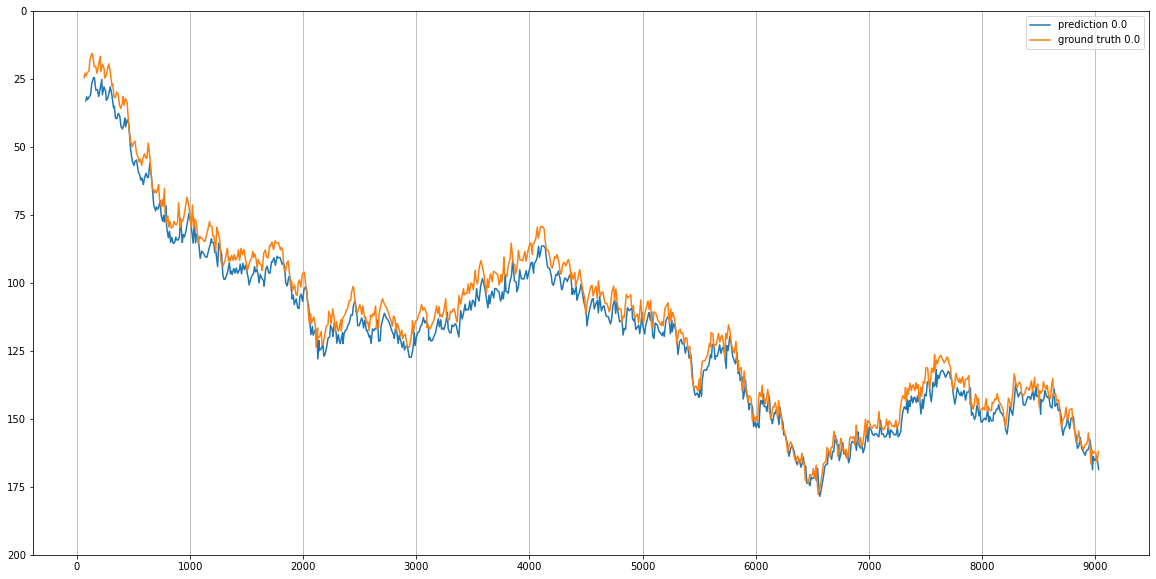
\includegraphics[width=\textwidth]{exp 5 test top}
  \caption{Experiment 5 with bottom particles as training set and top particles as testing set (shown)}
\end{figure}

\section{Experiments 6 and 7}
These two experiments are are similar to experiments 4 and 5. Experiment 6 randomly chooses 5 skyrmions for training and uses the rest for testing. Experiment 7 is divided in three parts, in each part either 5 skyrmions from top, centre or bottom are used for training and the rest for testing.

The results obtained and the plots obtained are very similar to experiments 4 and 5, hence I will not include them, but I can send them over if needed. Again, in these experiments, the indices for plotting have been fixed as well and the predictions have similar behaviour as the ground truth, but are sightly shifted.

\section{Recurrent Neural Network}
I have also explored the use of RNNs, but the results are not great yet as I have to tweak the hyperparameters and I am not sure my laptop can run a deep network. Each coordinate of each skyrmions is treated as a separate time series and and we can see that the predicted paths are quite similar to a drunken person walking around (figure \ref{fig:rnn}). This experiment still need quite a bit of work, so I will probably look into this a bit further this week.

\begin{figure}[h]
  \centering
  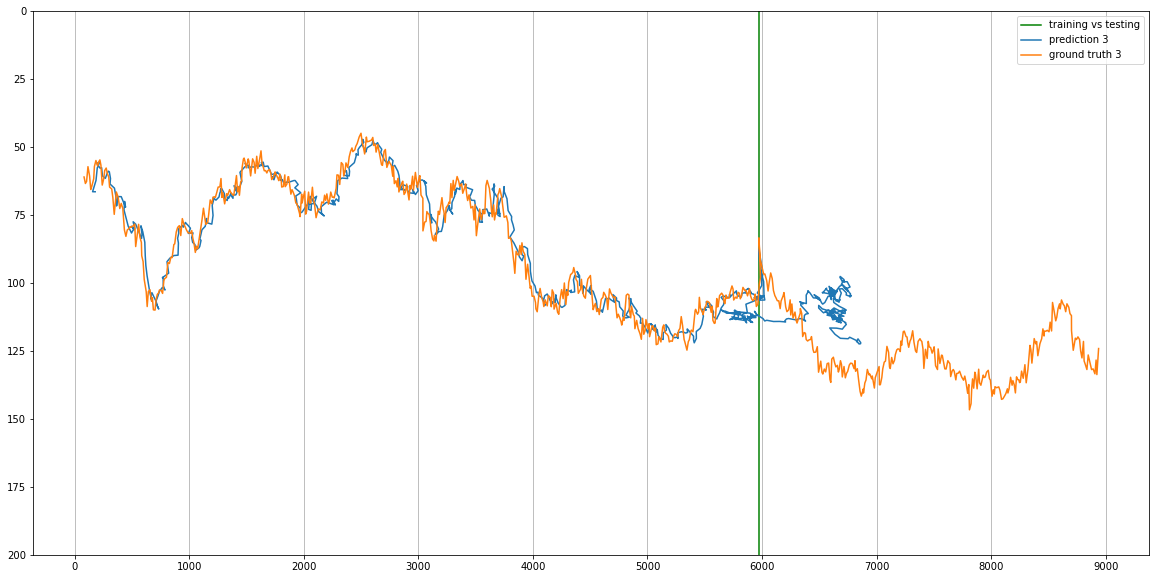
\includegraphics[width=\textwidth]{rnn}
  \caption{RNN Experiment}
  \label{fig:rnn}
\end{figure}

I also found a very interesting paper about trajectories prediction which discusses the use of what they call a "Social LSTM" for the prediction of human paths. A "Social LSTM" basically assigns a network to each person (or particle in our case) and at each time step we have a pooling layer which detects the nearby people (or skyrmions) so that particle interaction can be modelled as well. I need to read the paper more carefully, but it seems a very interesting idea to me. Let me know what you think Here is the link, as I cannot upload to DropBox since it's full: \href{https://cvgl.stanford.edu/papers/CVPR16_Social_LSTM.pdf}{Human Trajectory Prediction in Crowded Spaces}.

  
\end{document}